\begin{myprop}
	La \hspace*{5cm} des angles d'un triangle vaut 180\degree.
\end{myprop}


\begin{myexs}
	\begin{multicols}{2}
		\vspace*{1cm}
			Dans le triangle $ABC$, on a \\ %$\hat{A} + \hat{B} + \hat{C} = 180\degree$
		\vspace*{1cm}
		
		
			Dans un triangle isocèle, les deux angles à la base sont %égaux (ici 30\degree).
			\vspace*{2.5cm}
		
		
			Dans un triangle équilatéral, tous les angles sont %égaux et mesurent 60\degree.
			
			\vspace*{2.5cm}
			
			Dans un triangle rectangle, la somme des mesures %des angles non droits vaut 90\degree.
			
		\begin{center}	
		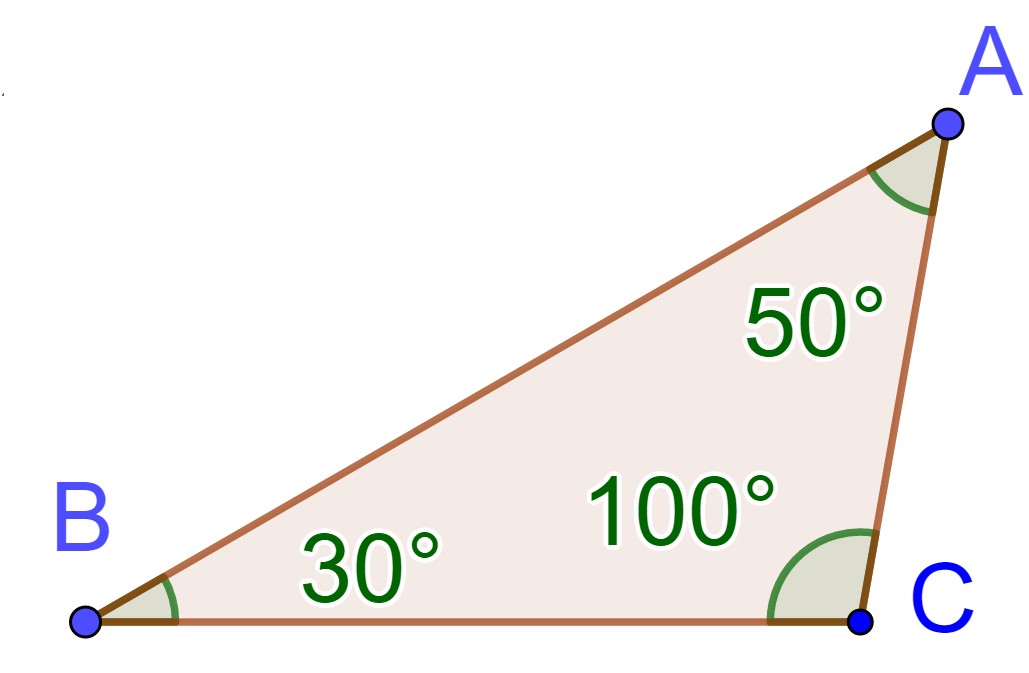
\includegraphics[scale=0.18]{quelconque}	
		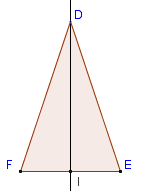
\includegraphics[scale=0.18]{isocele}	
		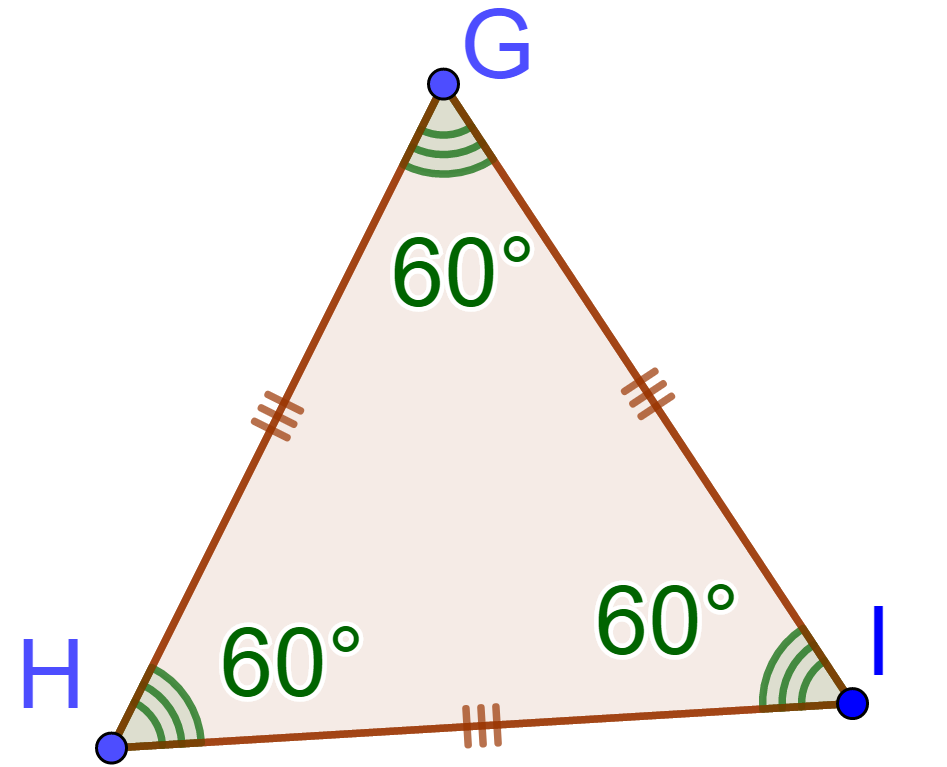
\includegraphics[scale=0.18]{equilateral}
		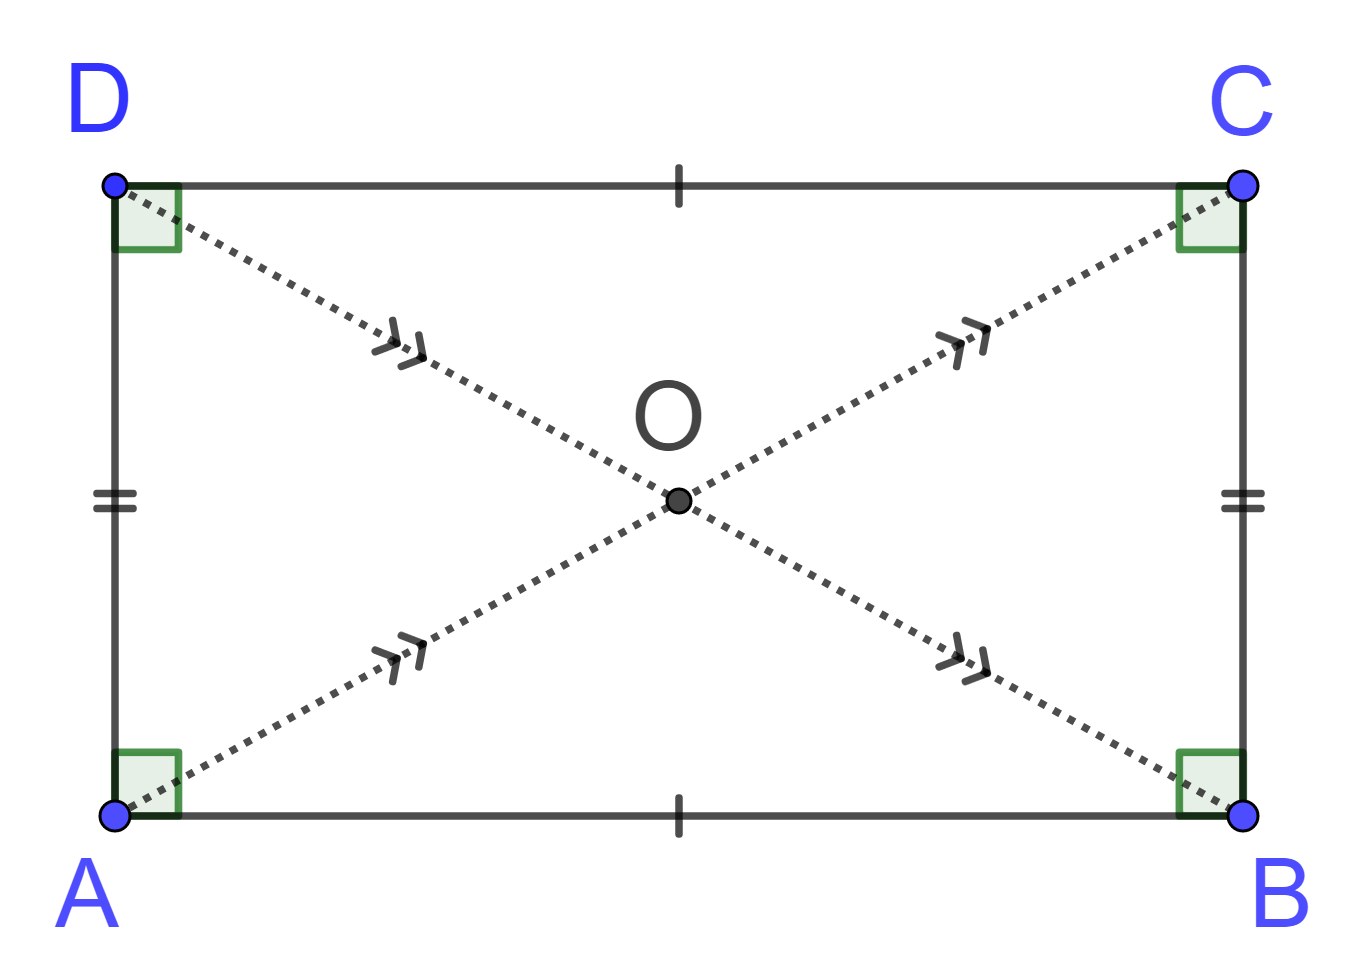
\includegraphics[scale=0.18]{rectangle}
		\end{center}
	\end{multicols}
\end{myexs}